\documentclass[10pt,compress,t,notes=noshow, xcolor=table]{beamer}

\input{../../style/preamble}
\input{../../latex-math/basic-math}
\input{../../latex-math/basic-ml}

% Additional TikZ libraries used by this deck (preamble already loads tikz with
% positioning/calc/shapes; we add modern arrow tips and shapes.geometric).
\usetikzlibrary{arrows.meta, shapes.geometric}

\usepackage{etoolbox}
\makeatletter
\newlength{\parboxtodim}
\patchcmd{\@iiiparbox}
  {\hsize}
  {\ifx\relax#2\else\setlength{\parboxtodim}{#2}\fi\hsize}
  {}{}
\makeatother

\setbeamersize{text margin left=0.3cm,text margin right=0.3cm}

% Colour palette for leakage diagrams (red = leaky, green = correct)
\definecolor{leakred}{HTML}{C0392B}
\definecolor{cleangreen}{HTML}{27AE60}
\definecolor{leakfill}{HTML}{FDEDEC}
\definecolor{cleanfill}{HTML}{E8F8F0}

% Armenian flag palette for the temporal-CV strip (3+ colour usage convention)
\definecolor{armred}{HTML}{D90012}
\definecolor{armblue}{HTML}{0033A0}
\definecolor{armorange}{HTML}{F2A800}

\begin{document}

\title{Applied Machine Learning}

% Title figure: validation-vs-deployment bar chart (TikZ, compiled from
% rsrc/leakage_title.tex into figure/leakage_title.pdf).
\titlemeta{
Data Leakage
}{
What it is, how to spot it, how to avoid it
}{
figure/leakage_title
}{
  \item Define data leakage and recognize its symptoms
  \item Identify the five major types: target, temporal, group, preprocessing, feature selection
  \item Apply the Golden Rule of preprocessing inside resampling
  \item Use a pre-deploy audit checklist before releasing a model
}


% =====================================================================
% Frame 2: Hook -- "The silent failure mode"
% =====================================================================
\begin{frame}{The silent failure mode}
\phantomsection\label{leakage-hook}

\textbf{Why this lecture exists.}

\medskip

\furtherreading{KAPOOR2023} surveyed ML applications across \textbf{17 scientific fields} and found data leakage in \textbf{294 papers}, often producing wildly overoptimistic conclusions and irreproducible findings.

\medskip

\begin{center}
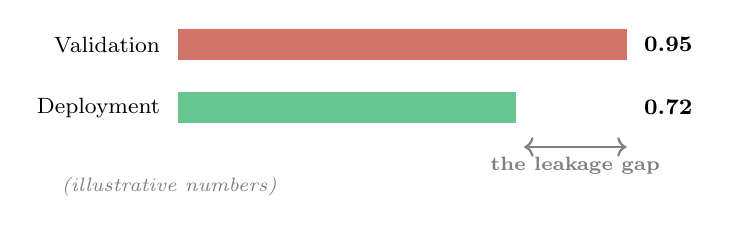
\begin{tikzpicture}[font=\footnotesize]
  % Top bar: reported performance (large)
  \fill[leakred!70]   (0,0) rectangle (5.7, 0.4);
  \node[left]  at (-0.1, 0.2) {Validation};
  \node[right] at (5.8, 0.2) {\textbf{0.95}};

  % Bottom bar: reproduced/deployment performance (smaller)
  \fill[cleangreen!70] (0,-0.8) rectangle (4.3, -0.4);
  \node[left]  at (-0.1, -0.6) {Deployment};
  \node[right] at (5.8, -0.6) {\textbf{0.72}};

  % Gap annotation
  \draw[<->, thick, gray] (4.4, -1.1) -- (5.7, -1.1);
  \node[gray, below, font=\scriptsize] at (5.05, -1.1) {\textbf{the leakage gap}};

  % illustrative tag
  \node[gray, anchor=west, font=\scriptsize\itshape] at (-1.6, -1.6) {(illustrative numbers)};
\end{tikzpicture}
\end{center}

\medskip

\textbf{The silent failure.} Cross-validation reports the same overconfident performance the leaky model produces. The leak is \emph{in the data}, not detectable from metrics alone.

\end{frame}


% =====================================================================
% Frame 3: What is leakage?
% =====================================================================
\begin{frame}{What is data leakage?}
\phantomsection\label{leakage-definition}

\textbf{Definition.} Any information from outside the training distribution that influenced training, or information that would not be available at the moment of prediction.

\bigskip

\textbf{Mechanism.} Data that \textit{would not be available} at prediction time leaks into the model during training.

\bigskip

\textbf{Symptom.} A large gap between cross-validation performance and held-out test performance, or implausibly good metrics.

\bigskip

\textbf{Why it is silent.} Cross-validation gives the same overconfident answer the model gives, because the leak is baked into the data, not into the procedure.

\end{frame}


% =====================================================================
% Frame 4: Leakage taxonomy (the big reference frame)
% =====================================================================
\begin{frame}{Leakage taxonomy: five types}
\phantomsection\label{leakage-taxonomy}

\renewcommand{\arraystretch}{1.25}
\footnotesize
% \raggedright in every column disables forced word-breaks; \arraybackslash
% restores \\ as row terminator (which \raggedright otherwise hides).
\begin{tabular}{|>{\raggedright\arraybackslash}p{2.1cm}|>{\raggedright\arraybackslash}p{2.6cm}|>{\raggedright\arraybackslash}p{3.9cm}|>{\raggedright\arraybackslash}p{2.6cm}|}
\hline
\rowcolor{gray!20}
\textbf{Type} & \textbf{Mechanism} & \textbf{Example} & \textbf{Fix} \\
\hline
\textbf{Target} & Feature contains future info & \texttt{last\_contact\_reason}\linebreak \texttt{= "cancellation\_call"} used to predict churn & Audit features; remove or recompute \\
\hline
\textbf{Temporal} & Random CV on time-ordered data & Shuffled daily-revenue series across folds & Blocked / forward-chaining CV \\
\hline
\textbf{Group} & Same entity in train and test & Patient ID appears in both folds & Group-aware split \\
\hline
\textbf{Preprocessing} & Transformer fit on full data & Scaler computed on train + test combined & Pipeline inside CV loop \\
\hline
\textbf{Feature selection} & Selecting features on full data & Ranking features by target correlation on full data, then splitting & Nested CV / selection inside fold \\
\hline
\end{tabular}

\medskip

\centering\footnotesize\itshape The next four frames develop types 1--4; feature selection is a forward reference to chapter~6.

\end{frame}


% =====================================================================
% Frame 5: Worked example -- Target leakage
% =====================================================================
\begin{frame}{Worked example: target leakage}
\phantomsection\label{leakage-target}

\textbf{Scenario.} Predicting customer churn from CRM records.

\medskip

\footnotesize
\begin{tabular}{|l|l|l|l|}
\hline
\rowcolor{gray!20}
\texttt{customer\_id} & \texttt{last\_contact\_reason} & \texttt{age} & \texttt{churned} (target) \\
\hline
A001 & technical support & 34 & 0 \\
A002 & \textbf{\textcolor{leakred}{cancellation\_call}} & 51 & \textbf{\textcolor{leakred}{1}} \\
A003 & billing question & 28 & 0 \\
A004 & \textbf{\textcolor{leakred}{cancellation\_call}} & 42 & \textbf{\textcolor{leakred}{1}} \\
A005 & technical support & 39 & 0 \\
\hline
\end{tabular}

\medskip
\normalsize

A naive model uses \texttt{last\_contact\_reason} and reports \textbf{0.98 AUC}. Looks fantastic.

\bigskip

\textbf{The catch.} At the moment we want to predict whether a customer \textit{will} churn, the value \texttt{"cancellation\_call"} does not exist for customers who have not yet churned. \emph{The feature is the answer.}

\medskip

\textbf{Detection rule.} Audit each feature by asking:
\begin{center}
\textit{Would this value exist at the moment of prediction?}
\end{center}

\end{frame}


% =====================================================================
% Frame 6: Worked example -- Temporal leakage
% =====================================================================
\begin{frame}{Worked example: temporal leakage}
\phantomsection\label{leakage-temporal}

\textbf{Scenario.} Forecasting daily revenue from prior days' data.

\medskip

\begin{center}
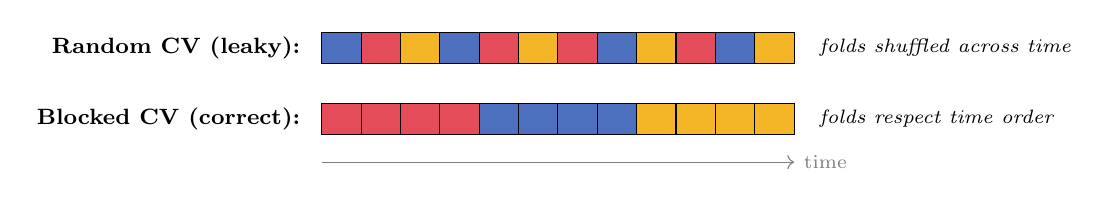
\begin{tikzpicture}[font=\scriptsize]
  % --- Top row: random k-fold (folds 1/2/3 shuffled across time) ---
  \node[anchor=east, font=\footnotesize] at (-0.15, 0.2) {\textbf{Random CV (leaky):}};
  \foreach \x/\f in {0/2, 1/1, 2/3, 3/2, 4/1, 5/3, 6/1, 7/2, 8/3, 9/1, 10/2, 11/3} {
    \ifnum\f=1 \fill[armred!70]    (\x*0.5,0) rectangle (\x*0.5+0.5, 0.4); \fi
    \ifnum\f=2 \fill[armblue!70]   (\x*0.5,0) rectangle (\x*0.5+0.5, 0.4); \fi
    \ifnum\f=3 \fill[armorange!85] (\x*0.5,0) rectangle (\x*0.5+0.5, 0.4); \fi
    \draw (\x*0.5,0) rectangle (\x*0.5+0.5, 0.4);
  }
  \node[anchor=west, font=\scriptsize\itshape] at (6.2, 0.2) {folds shuffled across time};

  % --- Bottom row: blocked CV, 12 cells colour-grouped (red | blue | orange) ---
  \node[anchor=east, font=\footnotesize] at (-0.15, -0.7) {\textbf{Blocked CV (correct):}};
  \foreach \x/\f in {0/1, 1/1, 2/1, 3/1, 4/2, 5/2, 6/2, 7/2, 8/3, 9/3, 10/3, 11/3} {
    \ifnum\f=1 \fill[armred!70]    (\x*0.5,-0.9) rectangle (\x*0.5+0.5, -0.5); \fi
    \ifnum\f=2 \fill[armblue!70]   (\x*0.5,-0.9) rectangle (\x*0.5+0.5, -0.5); \fi
    \ifnum\f=3 \fill[armorange!85] (\x*0.5,-0.9) rectangle (\x*0.5+0.5, -0.5); \fi
    \draw (\x*0.5,-0.9) rectangle (\x*0.5+0.5, -0.5);
  }
  \node[anchor=west, font=\scriptsize\itshape] at (6.2, -0.7) {folds respect time order};

  % time axis
  \draw[->, gray] (0, -1.25) -- (6.0, -1.25) node[right, font=\scriptsize] {time};
\end{tikzpicture}
\end{center}

\medskip

With random k-fold CV, day~50 may end up in training and day~49 in the test fold. The model uses \textbf{the future to predict the past}, then fails in deployment where the future is unknown.

\medskip

\textbf{Fix:} blocked CV or forward-chaining CV.

\end{frame}


% =====================================================================
% Frame 7: Worked example -- Group leakage
% =====================================================================
\begin{frame}{Worked example: group leakage}
\phantomsection\label{leakage-group}

\textbf{Scenario.} Predicting hospital readmission. Each patient has multiple visits.

\medskip

\begin{center}
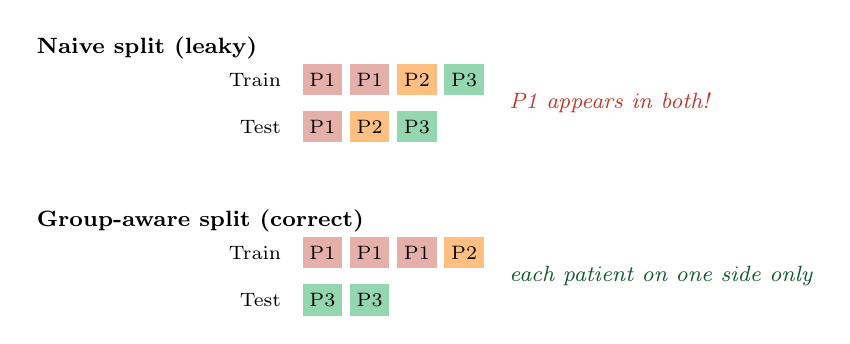
\begin{tikzpicture}[font=\scriptsize]
  % --- Naive split (leaky) ---
  \node[anchor=west, font=\footnotesize] at (-3.5, 0.8) {\textbf{Naive split (leaky)}};
  \node[anchor=east] at (-0.15, 0.4) {Train};
  \node[anchor=east] at (-0.15, -0.2) {Test};

  % Train row: rows from P1, P1, P2, P3
  \fill[leakred!40]    (0,0.2)   rectangle (0.5,0.6);  \node at (0.25,0.4)  {P1};
  \fill[leakred!40]    (0.6,0.2) rectangle (1.1,0.6);  \node at (0.85,0.4)  {P1};
  \fill[orange!50]     (1.2,0.2) rectangle (1.7,0.6);  \node at (1.45,0.4)  {P2};
  \fill[cleangreen!50] (1.8,0.2) rectangle (2.3,0.6);  \node at (2.05,0.4)  {P3};

  % Test row: rows from P1 (!), P2, P3
  \fill[leakred!40]    (0,-0.4)   rectangle (0.5,0);   \node at (0.25,-0.2) {P1};
  \fill[orange!50]     (0.6,-0.4) rectangle (1.1,0);   \node at (0.85,-0.2) {P2};
  \fill[cleangreen!50] (1.2,-0.4) rectangle (1.7,0);   \node at (1.45,-0.2) {P3};

  \node[leakred, anchor=west, font=\footnotesize\itshape] at (2.5, 0.1) {P1 appears in both!};

  % --- Group-aware split (correct) ---
  \node[anchor=west, font=\footnotesize] at (-3.5, -1.4) {\textbf{Group-aware split (correct)}};
  \node[anchor=east] at (-0.15, -1.8) {Train};
  \node[anchor=east] at (-0.15, -2.4) {Test};

  \fill[leakred!40]    (0,-2.0)   rectangle (0.5,-1.6);  \node at (0.25,-1.8) {P1};
  \fill[leakred!40]    (0.6,-2.0) rectangle (1.1,-1.6);  \node at (0.85,-1.8) {P1};
  \fill[leakred!40]    (1.2,-2.0) rectangle (1.7,-1.6);  \node at (1.45,-1.8) {P1};
  \fill[orange!50]     (1.8,-2.0) rectangle (2.3,-1.6);  \node at (2.05,-1.8) {P2};

  \fill[cleangreen!50] (0,-2.6)   rectangle (0.5,-2.2);  \node at (0.25,-2.4) {P3};
  \fill[cleangreen!50] (0.6,-2.6) rectangle (1.1,-2.2);  \node at (0.85,-2.4) {P3};

  \node[cleangreen!50!black, anchor=west, font=\footnotesize\itshape] at (2.5, -2.1) {each patient on one side only};
\end{tikzpicture}
\end{center}

\medskip

\textbf{Symptom.} CV reports 0.92 accuracy; held-out cohort of new patients reports 0.71.

\medskip

\textbf{Fix.} Split by group, not by row. In mlr3, assign a column the \texttt{group} role. Same logic applies to households, clinics, sessions, devices.

\medskip

\centering\footnotesize\itshape Leakage happens whenever CV folds violate the natural unit of generalisation.

\end{frame}


% =====================================================================
% Frame 8: Preprocessing leakage
% =====================================================================
\begin{frame}{Preprocessing leakage}
\phantomsection\label{leakage-preprocessing}

\textbf{The mechanism.} Any transformer that \textit{learns from data} (mean, variance, encoding mappings, PCA basis, k-means centroids) computed on the \emph{full} dataset already reflects the test rows. The model has seen the test data's footprint before predicting.

\medskip

\begin{center}
\begin{tikzpicture}[font=\scriptsize, node distance=0.4cm and 0.6cm]
  % LEAKY
  \node[rectangle, draw, fill=leakfill, rounded corners, minimum height=0.6cm] (full1) at (0,0.5) {Full data};
  \node[rectangle, draw, fill=leakfill, rounded corners, minimum height=0.6cm, right=of full1] (scale1) {Fit scaler};
  \node[rectangle, draw, fill=leakfill, rounded corners, minimum height=0.6cm, right=of scale1] (split1) {Split};
  \draw[-{Stealth[length=2mm]}, leakred, thick] (full1) -- (scale1);
  \draw[-{Stealth[length=2mm]}, leakred, thick] (scale1) -- (split1);
  \node[leakred, right=0.2cm of split1, font=\scriptsize\bfseries] {LEAK};

  % CORRECT
  \node[rectangle, draw, fill=cleanfill, rounded corners, minimum height=0.6cm] (full2) at (0,-0.7) {Full data};
  \node[rectangle, draw, fill=cleanfill, rounded corners, minimum height=0.6cm, right=of full2] (split2) {Split};
  \node[rectangle, draw, fill=cleanfill, rounded corners, minimum height=0.6cm, right=of split2] (scale2) {Fit scaler (train only)};
  \draw[-{Stealth[length=2mm]}, cleangreen!50!black, thick] (full2) -- (split2);
  \draw[-{Stealth[length=2mm]}, cleangreen!50!black, thick] (split2) -- (scale2);
  \node[cleangreen!50!black, right=0.2cm of scale2, font=\scriptsize\bfseries] {OK};
\end{tikzpicture}
\end{center}

\medskip

\textbf{Examples} (technique names; not developed here): mean imputation, feature scaling, target encoding, dimensionality reduction, k-means binning.

\medskip

You will encounter several of these in chapter~5 (feature preprocessing). The Golden Rule on the next slide applies to all of them.

\end{frame}


% =====================================================================
% Frame 9: The Golden Rule (centrepiece)
% =====================================================================
\begin{frame}{The Golden Rule}
\phantomsection\label{leakage-golden-rule}

\begin{center}
\fbox{\parbox{0.88\textwidth}{\centering\large
Every preprocessing step that \emph{learns from data} \\[0.2em]
must live \textbf{inside} the resampling loop.
}}
\end{center}

\medskip

\begin{center}
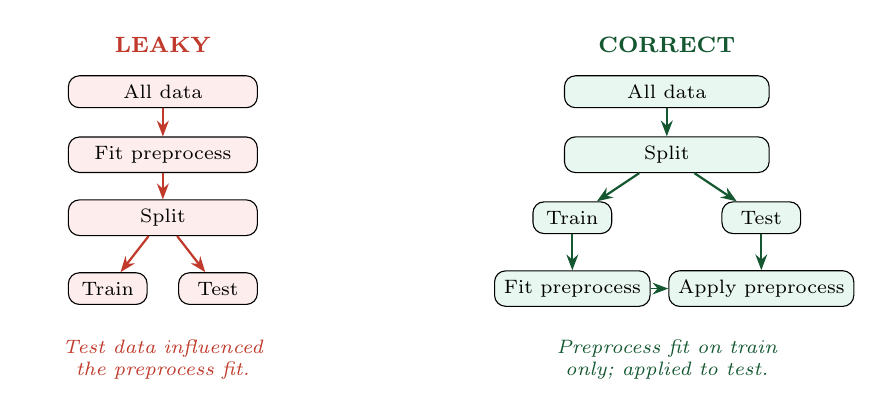
\begin{tikzpicture}[font=\scriptsize, every node/.style={align=center}]
  % --- Headers ---
  \node[font=\footnotesize\bfseries, leakred]            at (-3.2, 2.5) {LEAKY};
  \node[font=\footnotesize\bfseries, cleangreen!50!black] at (3.2, 2.5) {CORRECT};

  % --- LEAKY column (left) ---
  \node[rectangle, draw, fill=leakfill, rounded corners, minimum width=2.4cm] (L1) at (-3.2, 1.9) {All data};
  \node[rectangle, draw, fill=leakfill, rounded corners, minimum width=2.4cm] (L2) at (-3.2, 1.1) {Fit preprocess};
  \node[rectangle, draw, fill=leakfill, rounded corners, minimum width=2.4cm] (L3) at (-3.2, 0.3) {Split};
  \node[rectangle, draw, fill=leakfill, rounded corners, minimum width=1.0cm] (L4a) at (-3.9, -0.6) {Train};
  \node[rectangle, draw, fill=leakfill, rounded corners, minimum width=1.0cm] (L4b) at (-2.5, -0.6) {Test};
  \draw[-{Stealth[length=2mm]}, leakred, thick] (L1) -- (L2);
  \draw[-{Stealth[length=2mm]}, leakred, thick] (L2) -- (L3);
  \draw[-{Stealth[length=2mm]}, leakred, thick] (L3) -- (L4a);
  \draw[-{Stealth[length=2mm]}, leakred, thick] (L3) -- (L4b);
  \node[leakred, font=\scriptsize\itshape, text width=3.2cm] at (-3.2, -1.5) {Test data influenced the preprocess fit.};

  % --- CORRECT column (right) ---
  % R3a/R3b/R4/R5 spread to 2.4cm centre-to-centre so R4/R5 (min-width 1.4cm)
  % don't touch each other.
  \node[rectangle, draw, fill=cleanfill, rounded corners, minimum width=2.6cm] (R1) at (3.2, 1.9) {All data};
  \node[rectangle, draw, fill=cleanfill, rounded corners, minimum width=2.6cm] (R2) at (3.2, 1.1) {Split};
  \node[rectangle, draw, fill=cleanfill, rounded corners, minimum width=1.0cm] (R3a) at (2.0, 0.3) {Train};
  \node[rectangle, draw, fill=cleanfill, rounded corners, minimum width=1.0cm] (R3b) at (4.4, 0.3) {Test};
  \node[rectangle, draw, fill=cleanfill, rounded corners, minimum width=1.4cm] (R4) at (2.0, -0.6) {Fit preprocess};
  \node[rectangle, draw, fill=cleanfill, rounded corners, minimum width=1.4cm] (R5) at (4.4, -0.6) {Apply preprocess};
  \draw[-{Stealth[length=2mm]}, cleangreen!50!black, thick] (R1) -- (R2);
  \draw[-{Stealth[length=2mm]}, cleangreen!50!black, thick] (R2) -- (R3a);
  \draw[-{Stealth[length=2mm]}, cleangreen!50!black, thick] (R2) -- (R3b);
  \draw[-{Stealth[length=2mm]}, cleangreen!50!black, thick] (R3a) -- (R4);
  \draw[-{Stealth[length=2mm]}, cleangreen!50!black, thick] (R3b) -- (R5);
  \draw[-{Stealth[length=2mm]}, cleangreen!50!black, dashed] (R4) -- (R5);
  \node[cleangreen!50!black, font=\scriptsize\itshape, text width=3.2cm] at (3.2, -1.5) {Preprocess fit on train only; applied to test.};
\end{tikzpicture}
\end{center}

\vspace{-0.4em}

\footnotesize
\begin{itemize}\setlength\itemsep{0.15em}
  \item In \textbf{mlr3}: \texttt{po(...)} chains inside \texttt{as\_learner(...)} enforce this automatically when used with \texttt{resample()} / \texttt{benchmark()}.
  \item In \textbf{scikit-learn}: wrapping preprocessing in \texttt{Pipeline} (optionally with \texttt{ColumnTransformer}) enforces this when used with \texttt{cross\_validate} or \texttt{GridSearchCV}.
\end{itemize}

\vspace{-0.3em}

\centering\normalsize\textbf{\itshape When in doubt: split first, fit later.}

\end{frame}


% =====================================================================
% Frame 10: Spotting leakage -- heuristics + audit checklist (merged)
% =====================================================================
\begin{frame}{Spotting leakage: heuristics and audit checklist}
\phantomsection\label{leakage-detection}

\begin{columns}[T, totalwidth=\textwidth]

\begin{column}{0.48\textwidth}
\textbf{Detection heuristics}\\
\textit{\footnotesize (post-hoc, on a finished model)}

\medskip
\footnotesize
\begin{itemize}\setlength\itemsep{0.55em}
  \item \textbf{Big CV-test gap.} CV reports 0.95, holdout 0.80 $\Rightarrow$ suspect leakage.
  \item \textbf{Single feature too predictive.} Check its prediction-time availability.
  \item \textbf{Implausibly perfect performance.} Assume leakage until proven otherwise.
  \item \textbf{High-importance features.} Ask: ``would I have this value at the moment of prediction?''
\end{itemize}
\end{column}

\begin{column}{0.48\textwidth}
\textbf{Pre-deploy audit checklist}\\
\textit{\footnotesize (prospective, before shipping)}

\medskip
\footnotesize
\begin{itemize}\setlength\itemsep{0.25em}
  \item[$\square$] Split before any preprocessing fit?
  \item[$\square$] CV folds respect group structure?
  \item[$\square$] CV folds respect time structure?
  \item[$\square$] Each feature available at prediction time?
  \item[$\square$] CV vs final-test gap reasonable?
  \item[$\square$] Feature selection inside CV?
  \item[$\square$] No duplicate rows across the split?
\end{itemize}
\end{column}
\end{columns}

\end{frame}


\endlecture
\end{document}
